\subsection{Sequential Simulation}
We start by evaluating sequential simulation performance, in order to obtain a baseline for our comparison of parallel simulation performance.

\subsubsection{Queue}
\label{4-seq-Queue}
% explain what we did: fixed number of models (400, 600 & 800), increasing depth
For the first benchmark, we tested the effect of hierarchical complexity of the model in the performance of the simulator.
A set of three tests was performed, where each test has the same number of models but an increasing depth.
The results can be seen in Figure~\ref{fig:Queue_benchmark_seq}.
Since dxex performs direct connection on the model, there is no performance hit when the depth is increased.
Direct connection only needs to be done at initialization, so it is a one time cost that is negligible when simulation termination end time is sufficiently large.
Adevs, on the other hand, suffers from the increased depth, even though some similar (but not identical) optimization to event passing was made~\cite{adevs_opt}.
With every new hierarchical layer, routing an event from one atomic model to the next becomes more expensive, resulting in an increase in runtime.
\begin{figure}
	\center
	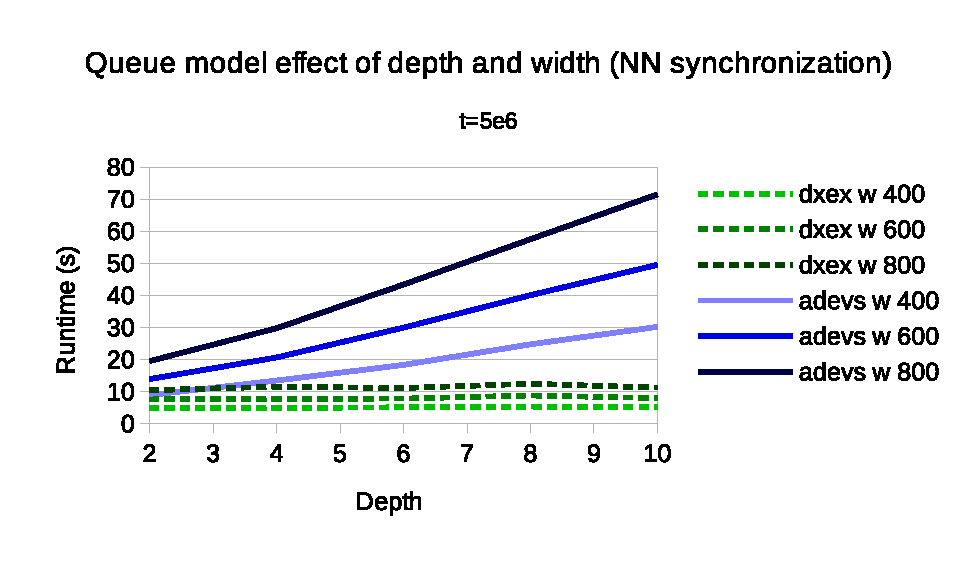
\includegraphics[width=\columnwidth]{fig/queue_fixed_sequential.eps}
	\caption{Queue benchmark results for sequential simulation.}
	\label{fig:Queue_benchmark_seq}
\end{figure}

\subsubsection{Interconnect}
\label{4-seq-Interconnect}
In the Interconnect model, we increase the number of atomic models, quadratically increasing the number of couplings and the number of external transitions.
As shown in Figure~\ref{fig:Interconnect_benchmark}, adevs now outperforms dxex by a fair margin.
Analysis showed that this is caused by the high amount of events: event creation is much slower in dxex than it is in adevs, despite dxex's use of memory pools.
To shield the user from threading and deallocation concerns dxex provides an event superclass from which the user can derive to create a specialized event type.
Copying, deallocation, and tracing are done at runtime, adding significant overhead when events happen frequently.
Profiling the benchmarks clearly shows the increasing cost of output generation and deallocation as the determining factor in the gap in performance.

\begin{figure}
	\center
	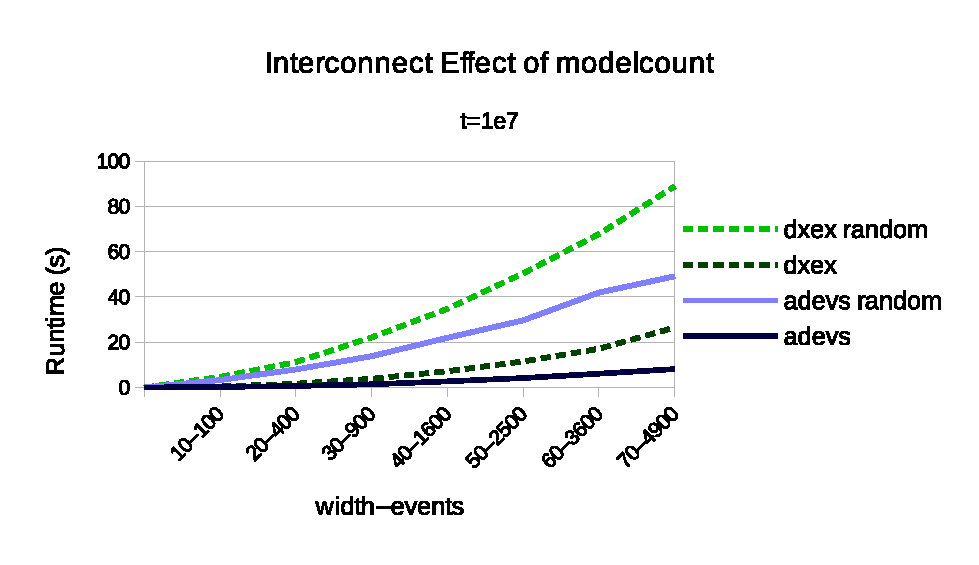
\includegraphics[width=\columnwidth]{fig/interconnect_sequential.eps}
	\caption{Interconnect benchmark results for sequential simulation.}
	\label{fig:Interconnect_benchmark}
\end{figure}

\subsubsection{PHold}
\label{4-seq-PHold}
The PHold model is very similar to the Interconnect model.
The biggest difference is that the amount of messages sent is much lower.
The number of events scales linear with the number of models, not quadratic.
Figure~\ref{fig:Phold_benchmark} shows that the performance of dxex and adevs are very close to each-other, with adevs slightly outperforming dxex.
\begin{figure}
	\center
	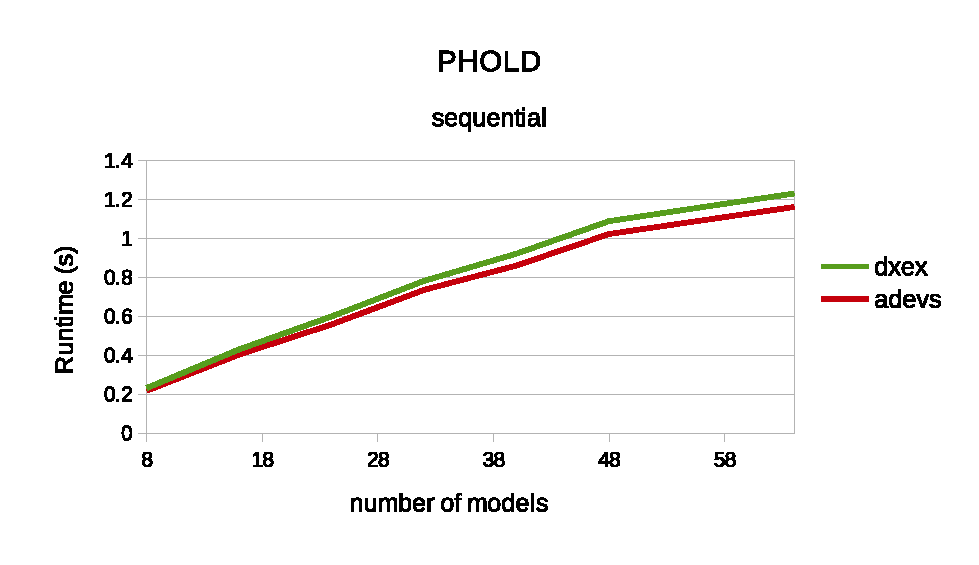
\includegraphics[width=\columnwidth]{fig/phold_sequential.eps}
	\caption{PHold benchmark results for sequential simulation.}
	\label{fig:Phold_benchmark}
\end{figure}
